%%%%%%%%%%%%%%%%%%%%%%%%%%%%%%%%%%%%%%%%%%%%%%%%%%%%%%%%%%%%%%%%%%%%%%%
%                                                                     %   
%    LateX template for UG final report                               %
%    Z. Wang 
%    Feb 2025
%    Updated on March 2026
%    University of Exeter                                             %
%                                                                     %
%%%%%%%%%%%%%%%%%%%%%%%%%%%%%%%%%%%%%%%%%%%%%%%%%%%%%%%%%%%%%%%%%%%%%%%
\documentclass[11pt,a4paper]{article}

\usepackage{amsmath}
\usepackage{amsfonts}
\usepackage{geometry}
\usepackage{graphicx}
\usepackage{fancyhdr}
\usepackage{setspace}
\usepackage{amssymb}
\usepackage{booktabs}
\usepackage{enumitem}
\usepackage{multirow}
\usepackage{titlesec} 

\usepackage{graphicx}
\usepackage{float}
\usepackage{subcaption}
\usepackage{hyperref}


% set table of content depth
\setcounter{tocdepth}{3} 
\usepackage[titles]{tocloft}

% set spacing 
\setlength{\cftbeforesecskip}{10pt}

% unticked checkbox
\newlist{checkbox}{itemize}{2}
\setlist[checkbox]{label=$\square$}
% ticked checkbox
\newlist{checkbox_t}{itemize}{2}
\setlist[checkbox_t]{label=$\text{\rlap{$\checkmark$}}\square$}

% Page layout settings
\geometry{
    a4paper,
    left=20mm,
    right=20mm,
    top=25mm,
    bottom=25mm
}

%%%%%%%%%%%%%%%%%%%%%%%%%%%%%%%%%%%%%%%%%%%%%%%%%%%%%%%%%%%%%%%%%%%%%%
%%%%%%%%%%%%%%%%%%%%%%%%%%%%%%%%%%%%%%%%%%%%%%%%%%%%%%%%%%%%%%%%%%%%%%
\begin{document}
\singlespacing  % Set the document to single line spacing
\thispagestyle{empty} % remove page number for the cover page

\begin{center}
    {\bf \LARGE Title of Your Project Topic}\\[0.5cm]
    \textbf{Your Name} \\[0.2cm]
    \textbf{Student ID:} 12345678 \\[1cm]
    % \textbf{Email:} youremail@exeter.ac.uk \\[1cm]
\end{center}

\section*{Abstract}

\noindent
This should be 200-250 word.
Cras laoreet eros a elit vehicula semper. Phasellus vitae condimentum felis. Suspendisse potenti. Suspendisse purus velit, convallis at bibendum sit amet, feugiat ut nulla. Vestibulum nec pharetra elit, vitae sodales enim. Maecenas tempor nisi quis posuere convallis. Sed fermentum rhoncus gravida. In pellentesque elementum enim, tristique ultrices lacus. Nunc scelerisque a nunc efficitur consectetur. Vivamus in quam quis sapien ullamcorper venenatis. In vestibulum sem orci. In hac habitasse platea dictumst. Interdum et malesuada fames ac ante ipsum primis in faucibus. Pellentesque dictum ornare metus, eu pellentesque quam luctus at.

\vspace*{\fill}

\begin{checkbox}
    % \item {\bf I have not used any GenAI tools in preparing this assessment.}
    \item {\bf I certify that all material in this dissertation which is not my own has been identified.}
\end{checkbox}

\vspace{1em}
{\bf\noindent Signature:} \hrulefill
\newpage

% table of contents
\tableofcontents
\thispagestyle{empty}
\newpage

% reset page number
\clearpage
\pagenumbering{arabic}

\section{Introduction}
The use of smart and connected medical devices has rapidly been adopted into the delivery of various healthcare services, which in turn, has lead to the rise of the Internet of Medical Things (IoMT). The IoMT is a subset of the Internet of Things (IoT) and includes various medical devices like remote heart rate monitors, patient temperature trackers, and continuos glucose monitors. Healthcare professionals are able to make use of IoMT systems in order to enable improved patient care and treatment delivery, through more efficient patient monitoring and personalised patient treatment. For example, data derived from IoMT devices was successfully used to predict the risk patients have for developing heart disease \cite{baseer2024healthcare}. However, as a result of this rapid integration of IoMT into modern healthcare, the attack surface for healthcare infrastructure has also become much larger for a variety of cyber threats. By the end of 2025, there had been 710 recorded healthcare data breaches, each of which affecting over 500 people \cite{hipaajournal}. Overall, these breaches impacted millions of patients, where sensitive medical records and other personal user data were exposed. This creates major concerns for the privacy of patients’ data, and their safety, as the IoMT becomes more integrated into the delivery of treatments and medications.
Within this rapidly evolving field, new vulnerabilities and cyber attacks are becoming an increasing concern for healthcare infrastructure, as IoMT devices are used in increasingly critical scenarios. Traditional defences such as firewalls alone, are no longer enough to ensure the security of these networks, one promising solution for this is the use of an Intrusion Detection System (IDS), which can pick up on malicious traffic missed by the firewall. Traditional, signature-based IDSs sometimes fail to detect more modern, and unknown attack signatures, which has lead to ML-based IDSs becoming a key area of recent research in network intrusion detection \cite{althubitiids, agarapneuralids, pramilaraniforest}. These ML-based IDSs are able to recognise the complex patterns found within network traffic flows and identify malicious activity, whereas signature based systems follow a list of set rules to identify malicious traffic. One downside of some ML-based IDSs is the lack of interpretability they have for the classifications they make, especially those that use complex deep learning models. This lack of interpretability limits the adoption of these newer IDSs into healthcare settings, this is because the safety and privacy of patients being treated using IoMT devices is critical, and any false flags for IoMT traffic could disrupt patients care and any missed malicious traffic could cause data breaches and further risk to patients.
To address this lack of of interpretability found in the more complex ML models, this projects focus will be on developing a Deep Neural Network (DNN) based IDS, and use Explainable Artificial Intelligence (XAI) techniques to verify the performance and accuracy of the model.
\subsection{Background}

\subsubsection{IoMT Architecture and Vulnerabilities}
IoMT systems tend to operate over three separate layers: the Perception (things) Layer, the Fog Layer, and the Cloud (Application) Layer. Illustrated in Fig~\ref{fig:IoMTLayers}. The Perception Layer comprises medical sensors, such as heart rate monitors, temperature monitors, and other wearable devices. This layer is vulnerable to physical tampering and data interference, which could lead to misdiagnosis and incorrect patient treatment.
The Fog Layer allows communication between devices and useful applications in the Cloud layer using protocols like Wi-Fi, MQTT, and Bluetooth. This layer faces threats such as DoS and DDoS attacks, which, if successful, will lead to disruption of patient treatment and put patient safety at risk. Data breaches are also a concern in this layer, where Man in the Middle attacks could compromise sensitive patient data.
Finally, the Cloud (application) layer is at risk of various software vulnerabilities as well as phishing and ransomware attacks, which could also lead to disruptions in healthcare delivery.
\begin{figure}[H]
    \centering
    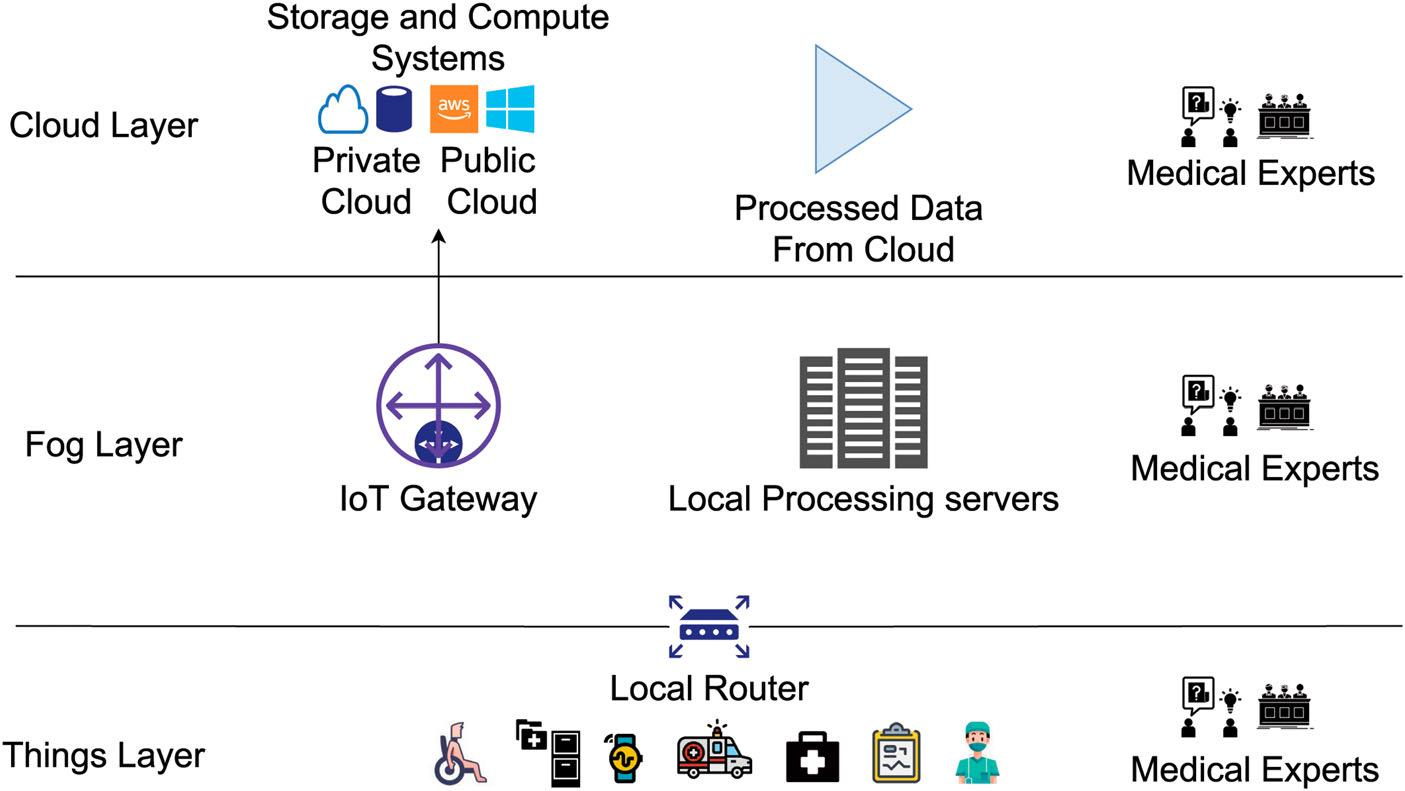
\includegraphics[width=0.75\linewidth]{images/iomt-architecture.jpg}
    \caption{Illustration of layers in an IoMT system. Source: \cite{razdan04072022}}
    \label{fig:IoMTLayers}
\end{figure}

%extned this to two pagessss then remove newpage
\newpage


\subsubsection{Evolution of Intrusion Detection}
Recent research focuses on using hybrid ML methods for intrusion detection, this is because these models such as Random Forest and deep reinforcement learning such as a Double Deep Q-Network (DDQN) \cite{da2019internet,lopez2020application} overcome the limitations of traditional signature based systems. These models show strong performance on test datasets like NSL-KDD \cite{nslkdddataset}, however these models would likely struggle to perform as well in real world healthcare settings because of the specific lightweight protocols used in IoMT systems such as MQTT. To address this issue, this project will use the CIC2024 IoMT dataset, this is because it provides a more realistic IoMT benchmark which simulates 40 different IoMT devices and modern attack types which are specific to IoMT networks.

\subsubsection{Explainable AI (XAI)}
Explainable Artificial Intelligence (XAI) includes tools that allow the decision making process of a deep learning model to be understandable to humans. This is mainly be in the form of showing which features a model has used when making a classification, and how it has used these features. This project will use Shapley Additive Explanations (SHAP), which is a method that assigns each numerical feature an importance value based on how it contributes to the model’s final output. Researchers in \cite{wang2020explainable}introduced a framework that uses SHAP alongside the NSL-KDD dataset \cite{nslkdddataset} in order to evaluate the performance of the IDS, this paper mentions the limitations of the framework, suggesting more datasets should be tested to improve the explainability of the system. The research applying these XAI techniques specifically to IoMT scenarios is currently limited, and this project focuses on this gap.

\subsection{Motivation}
ML based IDSs are able to recognise the
complex patterns found in network traffic to identify malicious activity, instead of
simple rule based systems. However, the lack of interpretability of these ML based
systems limits the widespread adoption, especially in healthcare setting where the
safety and privacy of both patients and staff are critical. To address this lack of
interpretability in more complex models, this project focuses on this critical gap by
developing a Deep Neural Network (DNN) IDS, and uses Explainable Artificial
Intelligence (XAI) techniques to verify the performance and accuracy of the model.
\newline
The main motivation behind this project is the requirement for transparency in safety
critical systems. Current ML-based IDS show solid performance, the reasons for
decisions they make are still very unclear, this reduces adoption in critical medical
environments because an incorrect classification could lead to disruptions in
healthcare delivery, or breaches of patients data. Existing IDS studies rely on the
use of general IoT datasets for training the models, these do not reflect the unique
traffic patterns which are found in IoMT networks, such as the use of lightweight
protocols like MQTT. This project uses the CIC2024 IoMT Dataset, this dataset has been
specifically created to benchmark and train IDS for IoMT traffic, it has been
generated using traffic collected from real IoMT devices. Although XAI techniques
such as SHAP and LIME have been used in general network security applications,
there has been little research applying these techniques specifically to IoMT
scenarios, this project aims to focus on that gap.

\subsection{Aims and Objectives}
The overarching goal of this project is to design, implement, and evaluate performance of an ML-based IDS, tailored to
IoMT network attack detection and using deep learning methods. Once this model has been implemented and it's performance
evaluated, XAI techniques (LIME or SHAP) will be applied to help explain how the model classifies different network attacks.
The results from these XAI techniques will then be discussed to verify that the model logically uses the features in the dataset
to make correct predicitons. The four primary objectives of this project are:
\begin{enumerate}
    \item Dataset Preparation - Obtain and apply preprocessing to the CIC2024 IoMT dataset, carry out any feature selection, encodings, and address the class imbalance, the dataset should be ready for any model training and have a balanced representation of attack classes for the model to train on.
    \item DNN Implementation - Design, Implement, and tune hyperparameters on a Deep Neural Network, which can then be validated using the reserved validation set of data. Ensuring the model reaches a macro F1-Score $\geq 0.8$ across the classes on the testing set.
    \item Integrate XAI - Apply SHAP to the now trained DNN to produce feature importance plots for each of the predicted classes.
    \item Explainability Analysis – Evaluate the outputs from the SHAP plots, comparing the feature importances to the real world attack signatures for each attack type. This can then confirm whether the model’s decisions are logical and consistent with network security knowledge.
\end{enumerate}


\section{Design and Methodology}
\subsection{Success Criteria}
The success of the project is measured by two overarching metrics: the performance of the Deep Neural Network, when detecting malicious network traffic, and the quality of the XAI explanations generated.
\begin{itemize}
    \item The primary metric for the performance of the IDS is the weighted macro F1-score, which has a target of 0.8 or above. This is obtained from the test set across all 5 of the attack categories learned by the model (including benign traffic). This metric was chosen over accuracy because of the large class imbalance found in the dataset, which is largely dominated by DoS and DDoS traffic, this imbalance would cause the accuracy to be a misleading metric of performance. Alongside the F1-Score, both precision and recall will also be used to analyse the tradeoff between false positives and false negatives, both of which are crucial issues when applying this IDS to healthcare systems. As well as this, a confusion matrix will be produced of all the classes in the test set, to identify the classes which the model is likely to incorrectly classify.
    \item To assess the explainability of the model, the SHAP plots will be examined to confirm whether features flagged by the model as most influential, are consistent with real world attack signatures. For example, a DoS attack is commonly identified through a high packet rate, the model should successfully pick up on this and the explainability plots should show this if the model works correctly.
\end{itemize}

\subsection{Pipeline Architecture}
The pipeline for the development of this IDS can be grouped into the following stages, also illustrated in Fig~\ref{PipelineDiagram}:

\begin{enumerate}
    \item Data loading and preprocessing: The raw CIC2024 IoMT dataset csv files are loaded into the notebook, cleaned, then transformed into a normalised and balanced training set which can be fed into a DNN. Validation and testing sets are withheld for hyperparameter tuning as well as final evaluation. The dataset split used in this project was 80% for training, 10% for validation, and 10% for testing.
    \item Model training and evaluation: The DNN is trained on the preprocessed training set, the validation set is then used to tune hyperparameters and prevent overfitting.
    \item Evaluation: The performance of the final model is then tested using the withheld testing set, using F1-score, precision, recall, and a confusion matrix to see how well the model performs on unseen data.
    \item XAI Analysis: SHAP is then applied on a sample of test predictions and the outputs of the plots are then compared to domain knowledge of the various attack types, this will reveal whether the model is using the correct information to predict network traffic type.
\end{enumerate}

\subsection{Development Methodology}
\subsubsection{Model Choice}
The model implemented in this project was a Deep Neural Network (DNN), this model was chosen because DNNs were amongst the strongest performers of all those tested in the original paper for the CIC2024 IoMT dataset. The DNN achieved strong F1 scores on both the binary and multi-class classification tasks, only being being beaten by the Random Forest classifier. DNNs have more complex internal architectures, making XAI integration more valuable, which is crucial for healthcare setting in this project.
\subsubsection{Dataset}
To train and benchmark the model implemented in this project, the CIC2024 IoMT dataset will be used, this was chosen over other commonly used IoT network traffic datasets such as the NSL-KDD and CICIDS2017. The CIC2024 IoMT dataset was specifically made to capture realistic traffic flows found in IoMT networks, it uses common protocols used by IoMT devices such as MQTT, Bluetooth, and Wi-Fi, which are not as common in these other datasets. It also simulates 18 different attack types which are focused on 40 simulated IoMT devices, making the attack surface large and varied. Finally, the dataset is easily accessible online for reproducing the results, it also does not contain any personal patient data or medical information, ensuring there are no ethical concerns with data privacy. Prior to applying any sampling pipelines or training the model, the dataset is split into training, validation, and testing sets, with 80% in the training set and 10% in both validation and testing sets.
\subsubsection{Class Imbalance Fix}
The CIC2024 IoMT dataset has 6 categories of network traffic: Benign, DDoS, DoS, MQTT, Recon, and Spoofing. There is a large class imbalance between these categories, with DDoS attacks making up 66.63\% of the dataset, and Spoofing attacks making up only 0.2\%. Due to the very small number of Spoofing attack samples, this category was dropped from the dataset. This was done because excessive oversampling would be needed to reduce the imbalance for this class would cause overfitting and misleading patterns, or undersampling large amounts of the majority classes would discard too much data. The distribution of the categories after removing the Spoofing category is shown in Fig~\ref{fig:TrainingSetPreSampling}. With the remaining 5 classes, a sampling pipeline is then applied to the training set, this involves undersampling the DDoS class, as well as using oversampling (SMOTE) to increase the number of samples for Benign, MQTT, and Recon traffic. After this pipeline is applied, we are left with a more balanced training set, where the largest class (DDoS) makes up 36.35\%, and the smallest (Recon) makes up 8.72\%, with the full distribution now shown in Fig~\ref{fig:TrainingSetPostSampling}. The validation and testing sets both retain the original, imbalanced distribution, this ensures that the evaluation of the model is carried out on real data and not synthetic samples.

\subsubsection{Choice of SHAP for XAI}
Following the initial project plan and literature review, the XAI section of the project was revised. Initially, both SHAP and LIME were to be used in order to evaluate the interpretability of the model. However, after testing both of these methods, the approach was altered focus only on SHAP. The main reason for this change was that SHAP provided more consistent explanations across the 5 categories, whereas when LIME was tested, the results tended to vary between tests. The SHAP framework also provided global and local interpretability and multiple types of plots to help analyse the results. To summarise, the project scope was adjusted to focus on the depth of the explanations, rather than focusing on two different explainability methods. SHAP’s Explainer was used in conjunction with a a random subset of $1,000$ instances sampled from the test set, this ensured a balance between representativeness of the dataset as well as compute time. The SHAP explainer was then used to generate the plots needed for the analysis used in the evaluation of the models interpretability.
\subsubsection{Feature Selection and Encoding}
Initially, the feature selection was to involve removing features with a near-zero variance. However, after initial testing, it was apparent that it lead to a decrease in the performance of the model when training on the dataset. This suggested that low variance features still had a significant impact on the models ability to learn from the dataset. As a result of this, this step was removed, and the full original set of features was then used to train the DNN. Numerical features were then scaled using a StandardScaler to ensure the DNN was able to converge during training, and categorical features were encoded with a LabelEncoder.


\section{Implementation}
\subsection{Dataset Pre-processing}
The original CIC2024 IoMT dataset is organised into multiple CSV files, each of these corresponds to a specific protocol and attack type. In order to work with this data, these files were first combined into a single combined dataframe with around $8.7$ million rows of data, each row containing 45 features. The spoofing class was then dropped from the dataset (discussed in section ???), prior to any additional processing, scaling or sampling. This reduced the classification task of the model from 6 categories, to 5 unique network traffic categories: DDoS, DoS, Recon, Benign, and MQTT.
The dataset was then split into training (80\%), validation (10\%), and testing (10\%) sets, this was done using the \texttt{traing\_test\_split} method found in the scikit-learn toolkit. Stratified sampling was also applied during this split to maintain the original imbalanced distribution, a random seed of 42 was also used at this stage to ensure the results were reproducible.
The attack category was encoded using scikit-learns’s \texttt{LabelEncoder}, and the remaining numerical feaures were standardised using the \texttt{StandardScaler}. Feature selection was tested by dropping the top 5 features whose variance was nearest to 0, however after training the model with this step, it was apparent that this reduced the performance of the model (mention in section ???).

Resampling of the dataset was carried out using a two stage sampling pipeline, with oversampling using SMOTE, followed by Random Undersampling:
\begin{enumerate}
    \item Oversampling was applied to Benign, MQTT, and Recon. These were oversampled using \texttt{SMOTE} with a random state of 42 to ensure reproducible results. The target sample number for Benign samples was $1.2$ million, $800,000$ for MQTT, and $600,000$ for Recon.
    \item Undersampling was applied to the majority class, DDoS, using \texttt{RandomUnderSamping} with a target sample number of $2.5$ million rows.
\end{enumerate}
The distribution of the categories prior to applying this pipeline is shown in Fig~\ref{TrainingSetPreSampling}. The final distribution after the pipeline has been applied is now shown in Fig~\ref{TrainingSetPostSampling}. Crucially, both the validation and testing sets were deliberately untouched by the pipeline, to ensure the evaluation of the model is based on real data, and synthetic samples don’t affect perceived performance.
\begin{figure}[H]
    \centering
    \begin{subfigure}{0.49\linewidth}
        \centering
        \includegraphics[width=\linewidth]{images/Training Set Before Sampling.png}
        \caption{Training set before sampling pipeline.}
        \label{fig:TrainingSetPreSampling}
    \end{subfigure}
    \hfill
    \begin{subfigure}{0.49\linewidth}
        \centering
        \includegraphics[width=\linewidth]{images/Training Set After Sampling.png}
        \caption{Training set after sampling pipeline.}
        \label{fig:TrainingSetPostSampling}
    \end{subfigure}
    \caption{Illustration of sampling pipeline.}
    \label{fig:SamplingPipeline}
\end{figure}

\subsection{DNN Implementation}
The Deep Neural Network (DNN) was implemented using \texttt{Tensorflow} in Python (version 3.12.3). After testing various architectures and iterative hyperparameter tuning, the final version of the architecture is shown in Table~\ref{tab:ModelArchitecture}.
\begin{table}[H]
    \centering
    \begin{tabular}{|l|l|l|l|}
        \hline
        Layer          & Type                & Size/Units & Activation \\ \hline
        Input          & Dense               & 45         & GELU       \\ \hline
        Hidden Layer 1 & Dense               & 256        & GELU       \\ \hline
        -              & Batch Normalisation & -          & -          \\ \hline
        -              & Dropout             & Rate = 0.3 & -          \\ \hline
        Hidden Layer 2 & Dense               & 128        & GELU       \\ \hline
        -              & Batch Normalisation & -          & -          \\ \hline
        -              & Dropout             & Rate = 0.2 & -          \\ \hline
        Hidden Layer 3 & Dense               & 64         & GELU       \\ \hline
        -              & Batch Normalisation & -          & -          \\ \hline
        -              & Dropout             & Rate = 0.2 & -          \\ \hline
        Output         & Dense               & 5          & Softmax    \\ \hline
    \end{tabular}
    \caption{Model architecture of DNN.}
    \label{tab:ModelArchitecture}
\end{table}
After building this model using Tensorflow’s \texttt{Sequential} object, it was then compiled with the Adam optimisier and a learning rate of $3\times 10^{-4}$. The loss function used was a categorical cross-entropy, which works well for multi class classification problems. The model was then allows to train on the dataset  for $75$ epochs, with a batch size of $2048$, early stopping was also allowed with a patience of $5$ epochs to help prevent overfitting and unnecessary computation time. The \texttt{ReduceLROnPlateau} callback was also applied with a factor of $0.5$ and patience of $5$ epochs, this helped stop the model getting stuck in local optima. The loss and accuracy curves for both the training and validation sets are shown in Figure~\ref{fig:LossAccCurves}, confirming that the model was able to converge whilst avoiding too much overfitting.
During validation, the epoch which yields the best loss was then saved, this saved model when then used throughout the evaluation and XAI analysis.
\begin{figure}[H]
    \centering
    \includegraphics[width=0.85\linewidth]{images/LossAccCurves.png}
    \caption{Loss and accuracy curves for training and validation data.}
    \label{fig:LossAccCurves}
\end{figure}
\subsection{XAI Integration}
After comparative testing between SHAP and LIME, it was apparent SHAP was more suitable for this project because the results generated by LIME were inconsistent across repetitions, and SHAP’s explainer was used instead. The trained model was used alongside a stratified sample of the test set (1000 samples), and a background dataset taken from the training set. Using a stratified sample meant that all of the categories were represented in the correct distributions found in the testing sets, and the explanations were not overwhelmed by the majority class (DDoS).
To begin with, a summary bar plot was generated to show the top $10$ features which had the highest SHAP values, meaning they had the largest influence on the models decisions. This plot also broken down the bars into 5 sections, showing how much influence the feature had on the prediction of each class.
Beeswarm plots were also generated, one for each class, these plotted the top $5$ features which influenced the model to predict the given class. These plots also showed the value of the features, which give a more in depth look at how the value of a feature either pushed the model toward or away from predicting the given class, such as a high packet rate pushing the model toward DoS or DDoS.
Using a sample size of $1000$ for the SHAP analysis yielded consistent results during testing, this value was settled on, because larger samples increased the computation time drastically. This sample size balanced the quality of the plots and the time it takes to produce them.

\section{Results, Testing, and Evaluation}
\subsection{Model Performance}
After training was complete, the best saved model was evaluated on the unaltered testing set, this set retained the original highly imbalanced dataset which was mentioned during the sampling pipeline. The testing set contained around $875000$ rows of data, which made up $10\%$ of the dataset.
The model achieved a macro average F1-score of $0.8603$, this exceeds the target score of $0.8$ set out in the objectives of the project which shows that the model is more than able tot distinguish between the $5$ attack categories presented in this classification task. This metric was chosen over just the accuracy because of the imbalanced nature of the test set mention previously. Looking closer at the results, shown in Table~\ref{tab:ClassificationReport}, the following can be seen across the classes:

\begin{table}[h]
    \centering
    \begin{tabular}{lcccc}
        \toprule
        \textbf{Class}        & \textbf{Precision}         & \textbf{Recall} & \textbf{F1-score} & \textbf{Support} \\
        \midrule
        Benign                & 0.9687                     & 0.9818          & 0.9752            & 23,034           \\
        DDoS                  & 0.8219                     & 0.8346          & 0.8282            & 584,663          \\
        DoS                   & 0.5463                     & 0.5242          & 0.5350            & 222,221          \\
        MQTT                  & 0.9945                     & 0.9920          & 0.9933            & 32,665           \\
        Recon                 & 0.9779                     & 0.9616          & 0.9697            & 13,140           \\
        \midrule
        \textbf{Accuracy}     & \multicolumn{4}{c}{0.7674}                                                          \\
        \midrule
        \textbf{Macro Avg}    & 0.8619                     & 0.8588          & \textbf{0.8603}   & 875,723          \\
        \textbf{Weighted Avg} & 0.7646                     & 0.7674          & 0.7659            & 875,723          \\
        \bottomrule
    \end{tabular}
    \caption{Model Performance Evaluation Using Precision, Recall, and F1-Score}
    \label{tab:ClassificationReport}
\end{table}
\begin{itemize}
    \item Benign: F1-score of $0.9752$, the model performs very well in identifying when traffic is benign, and has a low rate of false positives and false negatives for normal IoMT traffic.
    \item MQTT: Model achieved it’s best performance on this class, with an F1-score of $0.9933$, showing it can reliably detect when traffic belongs to the category of attacks over MQTT.
    \item Recon: F1-score of $0.9697$, model also had very strong performance on this class, showing it was able to distinguish between the other classes and reconnaissance attacks.
    \item DDoS: The model achieved an F1-score of $0.8282$ on this class, this performance is still good, but not as strong as the other classes. The recall was $0.8346$, and precision $0.8219$, suggesting the model confuses this category with other attack types. Suggesting the features used to identify DDoS and DoS are overlapping and causing misidentifications.
    \item DoS: This was the weakest class for the model, where it achieved an F1-Score of $0.5350$, showing that the model struggles to identify DoS attacks, which could be a result of similar feature values to DDoS attacks.
\end{itemize}
\begin{figure}[H]
    \centering
    \includegraphics[width=0.5\linewidth]{images/ConfusionMatrix.png}
    \caption{Confusion matrix showing models performance across all 5 classes.}
    \label{fig:ConfusionMatrix}
\end{figure}
To provide further insight into the misclassifications made by the model, the confusion matrix in Fig~\ref{fig:ConfusionMatrix} highlights where the model made mistakes. The majority of confusion is found between DDoS and DoS attacks. With $96,726$ DDoS being misclassifed as DoS, and $105,727$ DoS being misclassified as DDoS. This is most likely due to the similarities these attacks share, the model struggles to learn the boundary between the two with the current feature set. This will be explored further when the SHAP analysis is conducted, to see what features are leading to each of the predicted classes. One way this could be remedied is by grouping the DDoS and DoS attack categories into one larger class, as both of these attacks would have the same affect on an IoMT network by disrupting services. However, the low recall for DoS class would need improving for this IDS to be deployed, this is because large amounts of false negative flags for DoS would lead to large disruptions from these types of attack.
\subsection{Comparative Analysis}
The benchmark the performance of the DNN, it can be compared to the baseline performance of the DNN proposed in the original CIC2024 IoMT dataset paper. The model shown in this paper was tested on a 6 class problem, which is the closest comparison to this projects model, just without the small Spoofing class. The DNN proposed in the original paper achieved an F1-score of 0.665 \cite{dadkhah2024ciciomt2024}, which was significantly beaten by the model proposed in this project, which achieved an F1-score of $0.8603$. The model also outperformed the other model types tested in the original paper significantly, with the highest F1-score being from the Logistic Regression model, that achieved $0.694$.
The improvement in performance in this DNN is likely down to the resampling pipeline introduced during the pre-processing of the dataset, which the original paper makes not mention of. Making the training set have a more balanced class representation allowed the model to learn from a more general representation of IoMT network traffic. Another reason for the higher F1-score could be the more complex model architecture introduced, which was able to learn the complex underlying patterns in the dataset from the 45 numerical features.
\subsection{XAI Evaluation}
To carry out the SHAP analysis, $1,000$ samples were taken from the test set, this sample was stratified to ensure the class distribution was preserved and not affected by the large imbalance. Global plots were then produced, followed by a more in-depth look into per class feature importance plots.
\subsubsection{Global Feature Importance}
The global SHAP summary plot shown in Figure~\ref{fig:GlobalSHAPPlot} maps out the mean absolute SHAP values across all the predictions made. The top $10$ features with the highest mean absolute SHAP values are ranked from the most important at the top, to the least at the bottom.
\begin{figure}[H]
    \centering
    \includegraphics[width=0.85\linewidth]{images/GlobalSHAP.png}
    \caption{Loss and accuracy curves for training and validation data.}
    \label{fig:GlobalSHAPPlot}
\end{figure}
These results indicate that \texttt{Weight} is the biggest driver behind the model’s predictions, this reflects the role the amount of data in a network packet plays in the type of traffic it is, with weight effecting how likely the model classifies a packet as Recon.
\texttt{SRate} and \texttt{syn\_count} were also very large drivers behind predictions, heavily influencing the classificiations of DoS and DDoS, suggesting the amount of packets being sent over the network is able to determine whether it is a DDoS or DoS attack.
\texttt{IAT} (Inter-Arrival Time) was a also a large driver behind predictions, mostly for Recon traffic, suggesting the time between packets being sent significantly affects how likely it is to be a reconnaissance attack.
\subsubsection{Per-Class SHAP Analysis}
\begin{figure}[H]
    \centering
    \includegraphics[width=0.85\linewidth]{images/beeswarm_Benign.png}
    \caption{Beeswarm summary plot for Benign class.}
    \label{fig:BenignSHAP}
\end{figure}
Fig~\ref{fig:BenignSHAP} shows that high values of packet \texttt{Weight} suggest that the sample belongs to the Benign class, and when the weight is low, the model is more likely to classify it as one of the other traffic categories. Another notable feature here is the Inter Arrival Time (IAT), as the value of this feature increases, the model is more likely to classify a packet as benign. This aligns with expectations that genuine human generated traffic involves larger packet weights and time between packets. Whereas automated attacks like DDoS and DoS would have short time between packets and low weights.
\begin{figure}[H]
    \centering
    \includegraphics[width=0.85\linewidth]{images/beeswarm_MQTT.png}
    \caption{Beeswarm summary plot for MQTT class.}
    \label{fig:MQTTSHAP}
\end{figure}
Fig~\ref{fig:MQTTSHAP} shows that a high \texttt{ack\_flag\_number} causes the model to point toward a MQTT attack classification. The high number of acknowledgements made in attacks like MQTT floods are explain the importance of this predictor. The model has also learned that high values of \texttt{TCP}, which represents the average number of TCP packets in the window, point toward an MQTT attack. This could be because of the protocols reliance on TCP for it’s communication.
\begin{figure}[H]
    \centering
    \includegraphics[width=0.85\linewidth]{images/beeswarm_Recon.png}
    \caption{Beeswarm summary plot for Recon class.}
    \label{fig:ReconSHAP}
\end{figure}
Fig~\ref{fig:ReconSHAP} highlights that the model heavily relies on a high \texttt{fin\_count} to classify a sample as a recon attack, this aligns with reconaissance techniques like FIN scanning, where a large number of finish flags signifies malicious activity. On the other hand, a low \texttt{rst\_count} pushes the models prediction away from a Recon attack, and to another class, suggesting the model has learned to tell the difference between attacks with high reset counts like DoS.
\begin{figure}[H]
    \centering
    \includegraphics[width=0.85\linewidth]{images/beeswarm_DDoS.png}
    \caption{Beeswarm summary plot for DDoS class.}
    \label{fig:DDoSSHAP}
\end{figure}
In Fig~\ref{fig:DDoSSHAP} it can be seen that the most influential feature for classifiying samples as DDoS is SRate, a high SRate pushes the model towards a DDoS classification, this aligns with the known attack signature of DDoS attacks, where there are a high number of packets being sent. Furthermore, high values for the $ICMP$ and $TCP$ features push the model toward predicting DDoS, these features represent the number of ICMP packets and TCP packets being sent in a window respectively. A high number of TCP and ICMP packets aligns with the types of DDoS attacks which are within the dataset, with ICMP DDoS and TCP DDoS being amongst the largest specific attacks in the dataset.
\begin{figure}[H]
    \centering
    \includegraphics[width=0.85\linewidth]{images/beeswarm_DoS.png}
    \caption{Beeswarm summary plot for DoS class.}
    \label{fig:DoSSHAP}
\end{figure}
Fig~\ref{fig:DoSSHAP} gives insight into the limitations of this DNN, namely the confusion it has between DDoS and DoS classifications. It can be seen that the model relies a lot on \texttt{SRate} and \texttt{syn\_count} for the DoS class, similar to the DDoS class shown in Fig~\ref{fig:DDoSSHAP}, but incorrectly uses the features when looking at DoS. A high \texttt{Srate} pushes the model away from a DoS prediction, and high ICMP and TCP values pushes it away from DoS, these results are no the ones expected for this class. The feature overlap with SRate could be the main reason for the limited boundary between the two, and future models would benefit from incorporating source and destination IP’s to see whether the packets are coming from one source, or many.

\section{Reflection and Conclusion}
\subsection{Critical Reflection}
\subsubsection{Successes}
Throughout the course of this project, all of the primary objectives set out in the beginning have been met. Firstly, the DNN achieved a macro average F1 score of $0.8603$ during it’s evaluation on the test set, this is significantly more than the target score and shows the model successfully learned to classify the $5$ classes presented in the dataset. The model excelled in identifying MQTT attacks, Benign traffic, and Recon traffic, with excellent F1-scores on these $3$ classes. Furthermore, this performance was significantly better than the benchmark F1-score presented in the CIC2024 IoMT paper, in which the DNN achieved an F1-score of 0.665. This improvement is mainly a result of the sampling pipeline applied to the dataset, which allows the model to generalise rather than overfit to the imbalanced training data.
The decision to discard the Spoofing was crucial in improving the performance of this model. The Spoofing class only contained $17791$ samples, which was very small in comparison to the largest class, DDoS, which contained over $5846623$. Attempting to oversample to compensate for this difference would not reflect real world data and skew the training, and undersampling would mean lots of data would be discarded. The decision to solely focus on SHAP for the XAI analysis, rather than both SHAP and LIME was also a well justified alteration to the initial goals of the project. The instability in results produced by LIME would have conflicted with the projects aim to maximise trust and interpretability of the IDS. Choosing to just use SHAP allowed for more in depth and reliable results.
The SHAP analysis gave insight into the models strengths, with the per class beeswarm plots showing how the model learned feature patterns that align with existing cybersecurity knowledge of attack types. For example, a high \texttt{SRate} as well as high \\texttt{ICMP} and \texttt{TCP} packet counts pushed the model toward predicting a DDoS attack. This result helps assure that the model is generalising about the attack signatures in IoMT network traffic, and not just exploiting patterns specific to the training data.

\subsubsection{Limitations}
The main drawback of the model in this IDS is the poor performance when classifying DoS attacks, for which the F1 score was only $0.5350$. This becomes more apparent in the confusion matrix in Fig~\ref{ConfusionMatrix}, where $105,727$ DoS instances were incorrectly classified as DDoS. Similarly, $96,726$ DDoS samples were incorrectly classified as DoS attacks, making it clear that the DNN struggled to find a clear boundary between the two classes. Using the SHAP summary plots found in Fig~\ref{fig:DoSSHAP} and Fig~\ref{fig:DDoSSHAP}, it is clear that the model relies heavily on $SRate$ and $syn\_count$ for both of these classes, but with the directions in the SHAP plots inverted. The SHAP plot for DoS shows this inverted direction where a high \texttt{SRate} pushes the model away from predicted DoS, this is not expected behaviour as this attack type should be characterised by the opposite value. The main reason for this is the CIC2024 IoMT datasets lack of source as well as destination IP addresses, having this within the feature set would allow models to find this boundary between DoS and DDoS traffic, where DoS comes from a single source, and DDoS comes from many. This limitation would need to be a addressed in a deployment of this IDS to an IoMT network, because the high false negative rate would lead to significant disruption to healthcare services due to missed DoS attacks.

\subsection{Conclusion}
\subsection{Future Directions}






\newpage
%%%%%%%%%%%%%%%%%%%%%%%%%%%%%%%%%%%%%%%%%%%%%%%%%%%%%%%%%%%%%%%%%%%%%%
%
%    REFERENCES
%
%%%%%%%%%%%%%%%%%%%%%%%%%%%%%%%%%%%%%%%%%%%%%%%%%%%%%%%%%%%%%%%%%%%%%%
\bibliographystyle{IEEEtran}
\bibliography{main.bib}

%%%%%%%%%%%%%%%%%%%%%%%%%%%%%%%%%%%%%%%%%%%%%%%%%%%%%%%%%%%%%%%%%%%%%%
%
%    Appendices
%
%%%%%%%%%%%%%%%%%%%%%%%%%%%%%%%%%%%%%%%%%%%%%%%%%%%%%%%%%%%%%%%%%%%%%%
\appendix
\section*{Appendix A}
\addcontentsline{toc}{section}{Appendix A} % add Appendix A to contents line

\end{document}
